% {\color{red}asdf}

\newtheorem{DEF}{Definition}

%=====================================================================================
\chapter{Introduction}
%=====================================================================================

In these days, Continuous Integration (CI) is more often used in larger projects, where multiple developers are working on one and the same software product. This process ensures fast software development, called eXtreme Programming (XP), known as agile software development methodology. The methodology is mainly used to accelerate the development, nevertheless, development of software may be disrupted in various other ways. Nowadays, although this type of software development has many disadvantages, it is still much more often used on larger projects. The progress of the development may not be reached with a continuous integration which guarantees less disorder and failures. You may also know that the continuous integration is a part of the following open-source projects e.g. Facebook, Twitter, Mozilla. These projects use one of many famous continuous integration service Travis CI. Excluding Travis CI, there are plenty of other continuous integration services you may heard about, such as Jenkins, TeamCity, CircleCI, GitLab CI, Codeship and so on.\\

The software development process requires many code checking tools after every single code change in the source code. For as much as with every single change of code, there is a possibility to add, fix, derange or deteriorate any parts of the software product. These tools provide an automated code review and they afford a quick feedback by which they try to prevent these code impairments. Feedback about his adjustment is sent to the developer, who has made the change in the code. The automated process which provides the code review does not bother with executing a huge amount of tests. Above mentioned process is conducted via continuous integration server, which compiles the code, runs scripts and tests. The results are aggregated and the feedback is given to the developer who has made this code change. Continuous integration server is invoked every single time after any change is fetched in the source code and he had to execute the stated acts which are predefined. In next chapters we describe in details how does this workflow work and what steps are required to run.\\

The essence of this work is about the basics of continuous integration and its fundamentals. This thesis attempts to explain how the fundamentals of continuous integration and automated code review work. It describes how it is integrated to the software development, and how it works on an extensive project nowadays. Examples will be based on open-source project e.g. ManageIQ, which is a cloud manager founded by Red Hat, Inc. The development process of the ManageIQ rests in agility and stability of the progress. These main factors of the development process could not be reached without a quick feedback to the developers working on project about their changes, that are submitted to the software product.

%=====================================================================================
\chapter{Continuous Integration and Automated Code Review}
%=====================================================================================

In the face of the fact that continuous integration and automated code review are used in a lot of projects, it is still an unknown part of software development. Despite CI rising as a big success story in automated software engineering, it has received almost no attention from the research community \cite{COPE}. There are only a few researches describing this part of development how is it deployed, managed and used. Development analysts are not giving an adequate attention to this part of software development. They are usually describing it as a common part of development in a software development process. This part is concerning to extreme programming due to fast code change deployment. This development technique is very adaptive and still more and more open source projects are using it. There are many developers relying on this type of software development which helps them rapidly. This chapter will give you a detailed view of the modern in-use software development methodology which is still in evolution.

%=====================================================================================
\section{Continuous Integration}
%=====================================================================================

Continuous integration (CI) has a key role in the software development process consisting of a few certain unavoidable steps which will be described later in next subsections. CI is believed to be an effective way to integrate the source code faster and certify the result of such cooperation, hence an important component of modern software parallel development environments \cite{ResultsOfCIbuild}. Everything begins at the moment, when one developer who has made changes in a source code of the software product is trying to commit them into the software product. The process of continuous integration has begun at this point and lasts until feedback is sent back to the developer. These stages of continuous integrations are proceed every time after the CI server has detected a change in a version control repository. This automation has a lot of benefits which are necessary to keep the software product without any kind of defects. Many of them are detected in time and reported back to the developer as a corrupted source code. Not a few developers may think that the continuous integration is only about compiling a source code and launching tests. In the next subsections, we will present the steps of the continuous integration and describe these individual phases in detail.\\

To imagine the process, there is a illustration about the components and their connections in the process of continuous integration in Figure \ref{fig:cocis}. The image illustrates situation when \textit{Developer 1} commits changes to the version control repository. The CI server detects this change and provide a feedback about the change back to the \textit{Developer 1}. The \textit{Developer 1} can review informations about change that he made in the given feedback, e.g. tests results.

\begin{figure}[H]
    \centering
    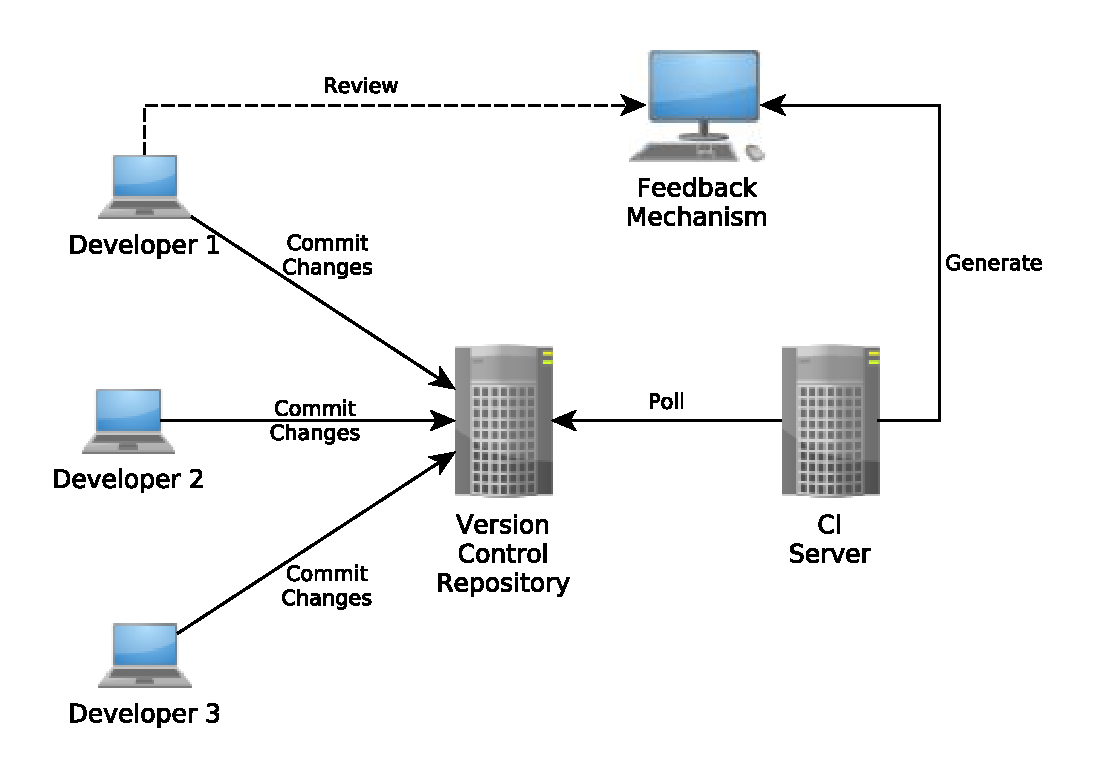
\includegraphics[scale=0.6]{yEd/components_of_CI_system.eps}
    \caption{Components of continuous integration system \cite{CIbook}.}
    \label{fig:cocis}
\end{figure}

%=====================================================================================
\subsection{Demands of Continuous Integration}
%=====================================================================================

The minimal requirements for a good software development of a project where multiple developers are working on the same project are a version control repository and a continuous integration server. The version control system guarantees a software configuration management which is required for the continuous integration. The meaning of the version control system is very important. You cannot manage changes that developers had made in the source code without a version control system. The version control system has a very positive impact on the developing project. The system offers a history of changes which may be highly useful if a rollback is desired. Besides the history of changes, this system may save more other information about the source code, e.g. who did the change, when was the change created, etc. In addition, the version control system represents a primary source for the project source codes. This type of project setup is much more often used these days than in the past. Nearly every project has its own version control system which is provided by a repository hosting service.\\

A CI server has a huge advantage. This is a reason why it is highly recommended. It depends on the developer, how does he deploy the CI server. With the CI server, he does not have to bother with such many scripts for the automation. Nevertheless, as he decides how the CI server will be established, the system must contain these features. To facilitate the process of continuous integration, the system must support services as polling version control system, retention of build history, launching predefined steps such as scripts and tests. Furthermore, the system should offer an opportunity to send a feedback back to the developers. This server executes a series of actions or steps taken in order to achieve a particular end of CI. The next subsection will determine and state these fundamental steps of the continuous integration scenario and describe and illustrate them in detail.

%=====================================================================================
\subsection{Stages of Continuous Integration}
%=====================================================================================

The stages of CI insure code inspection and code integration. Before we begin, we need to clarify certain concepts which will be used later. To understand these steps, we need to understand what is the difference between \textbf{a build}, \textbf{a private build} and \textbf{an integration build}.

\begin{DEF}
A build may refer to a set of activities performed to generate, test, inspect, and deploy software \cite{CIbook}.
\end{DEF}

\begin{DEF}
A private build define a process in which a software developer runs the build on his local machine to ensure that the changes he made work before he commits them into a version control repository.
\end{DEF}

\begin{DEF}\label{def:IntegrationBuild}
An integration build is the act of combining software components (programs and files) into a software system \cite{CIbook}.
\end{DEF}

Figure \ref{fig:IntegrationBuild} mentions the before stated Definition \ref{def:IntegrationBuild} which depicts the result of combination individual parts (components) of the software into a single software system. The transformation process that integrate these software components together into a one unified entity is called as an integration build.

\begin{figure}[H]
    \centering
    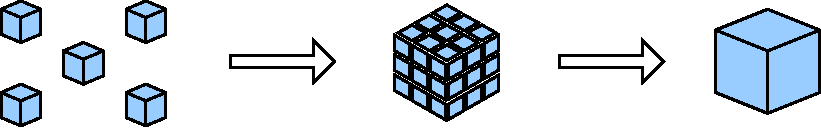
\includegraphics[scale=1]{img/system_integration.pdf}
    \caption{Integration build.}
    \label{fig:IntegrationBuild}
\end{figure}


Now as we know what are these concepts we will illustrate the basic stages of continuous integration. To describe it properly, imagine that we have a group of developers working on the same project using a version control system where the source code of the software product is held, and they use a continuous integration service. The stages of continuous integration are the following:

\begin{enumerate}

    \item \textbf{The change}\\[0.1em]
          One developer who wish to make a change, adjustment, improvement or to create a new feature in the software product has to clone the remote version control repository to his local computer to download the source code of the software product. At this point, he has a local version control repository in which he will do the changes he would like to. After a change is made, the change is only in a local repository and the developer would like to commit it into the remote repository. Before publishing the change, he has to run a private build. The developer has to publish the change he made which is a request for an approval of the change ready to merge into a specific branch on the remote repository. These not merged changes are published on the remote version of the control repository.\\[0.1em]
          By committing changes to the version control repository a continuous integration server is invoked. The continuous integration server polles the version control repository when a change is detected, after this poll a reaction occures.

    \item \textbf{The reaction}\\[0.1em]
          When a change is detected it invokes a continuous integration server to execute a few tasks. The tasks are predefined in a build script which has to integrate the change with the rest of the source code of the software product. The script provide source code compilation, database integration, testing and code inspection. The execution of the script is referred to as an integration build.\\[0.1em]
          This stage of continuous integration usually includes also code verification. It finds defects or errors made by developer, e.g a compilation fail, tests failures etc. The errors are detected by tests which should have high code coverage. A number of errors in this stage can be reduced by launching a private build which may be less complex compared to launching the build script. Passing this stage depends on success of the build script which must be success on 100\%.

    \item \textbf{The feedback}\\[0.1em]
          The continuous integration server generates a feedback associated to the results of the build which is assigned to this change and it might be sent to the author of the change. There is log information generated every time, by passing the reaction stage, and it is held and assigned to the change. Feedback is given to the developer in a certain predefined form, e.g. email with failures only. The log file is saved on the continuous integration server where there is an overview about the builds and their stats.

    \item \textbf{The waiting}\\[0.1em]
          This stage is the end of the process. It stands for continuous polling of  the version control repository waiting for a new change. Detecting a change will cause launching the stages from the beginning.

\end{enumerate}

%=====================================================================================
\subsection{Continuous Integration Server}
%=====================================================================================

If the software development proceed to use continuous integration in the workflow it might have a configured CI server. The principal sense of a continuous integration server is to get rid of a manual integration build. The configuration of the CI server depends on source code verification requirements and on type of polling. The CI server can also provide an additional automation for necessary essentials to the development such as integration, deployment, etc.\\

The continuous integration system is based on automation that is conducted by CI server. Automation is an act, when manual tasks are united and executed together in order to simplify the execution of manual tasks. Nowadays, in software development automations can be found in different parts of software development. It helps to accelerate the development process. In a CI system, there are different types of builds and mechanisms used for the automation.

\subsubsection{Polling}

We can distinguish several types of build mechanisms such as on-demand, scheduled, poll for change and event-driven mechanism \cite{CIbook}. The simplest automated mechanism, on-demand mechanism, can be done by a single script and it helps to get rid of tasks repetition executed by the developer. The on-demand mechanism is an user-driven process in which someone manually initiates an integration build \cite{CIbook}. Scheduled mechanism is a planned event accomplished by CI server in predefined time. In the situation where multiple developers are frequently working on a product during the day, the best choice for a build should be to plan it in night. The scheduled type is used particularly when an advanced build of the software product is needed to be done. Scheduled processes are driven by time, for instance, so that it runs on an hourly basis, whether or not a change has occurred \cite{CIbook}.\\

Poll for change mechanism and event-driven mechanism differ only in a way of invoking. Poll for change mechanism uses a periodic time for a change polling and the event-driven mechanism is time independent mechanism which is invoked by a version control repository. In a poll for change mechanism, a process wakes up in a regular intervals and checks for changes to the version control repository, if changes are detected an integration build is ran \cite{CIbook}. The event-driven mechanism is triggered by a version control repository, if change was detected by version control repository than it initializes the build script. Only in these two mechanisms there is a polling service which is sectionalized into two different types.\\

Types of polling can be divided into two parts - time dependent polling and change dependent polling. The CI server with time dependent polling is configured to check the version control repository for a new change in predefined periodic time intervals e.g. every 10 minutes. Contrawise, the CI server with change dependent polling is invoked with every single action which is a change in a version control repository via an informative message about the current action sent to the CI server. This message including event stats is triggered on a specified event in the version control repository which must support this feature.\\

Time dependent polling is mostly used in general due to inadequacies such as missing event triggering in the version control repository. Due to this fundamental feature some of CI servers has to have  periodic polling on time. The main disadvantage is the time taken by downloading the actual source code from the repository. After the download is complete, the changes are still unknown, a comparison must be done between the latest and the last source code for the purpose of obtaining the new changes. Change dependent polling downloads only the real change towards the actual source code status made in the repository. If the version control system can support this feature the source code synchronization is much more faster and efficiently done.

%=====================================================================================
\subsection{Build Script}\label{build_script}
%=====================================================================================

Instigation of CI system begin with a change in the version control system resulting in build script execution. Transforming sources into a system and simultaneously providing a review about the transformation is an intricate process also known as continuous integration, delivery and deployment. A CI system uses a build script allowing build automation, which includes every predestined statement to execute. This automation had a magnificent demand in software development. To get rid of constantly repeated actions for the purpose to accelerate the software development a build script was created. The principal script consists of a set of subscripts, which divide the automation into segments that are bound to themselves according to the execution order. Segments are shown in order in Figure \ref{fig:lpobs}. It shows the logical parts of a build script. Script performs a build also called as a software build which is not just about the source code compilation and tests launch. These various smoothly executed parts construct a functional unit of the software product. A working function unit congregation leads to working software deployment as the final step of CI. The script warrants simplification because of the developers adjust the source code and they are able to gain instant feedback about their work. As Martin Fowler said \uv{Get everything you need into source control get it so that you can build the whole system with a single command.} \cite{MartinFowler}.

\begin{figure}[H]
    \centering
    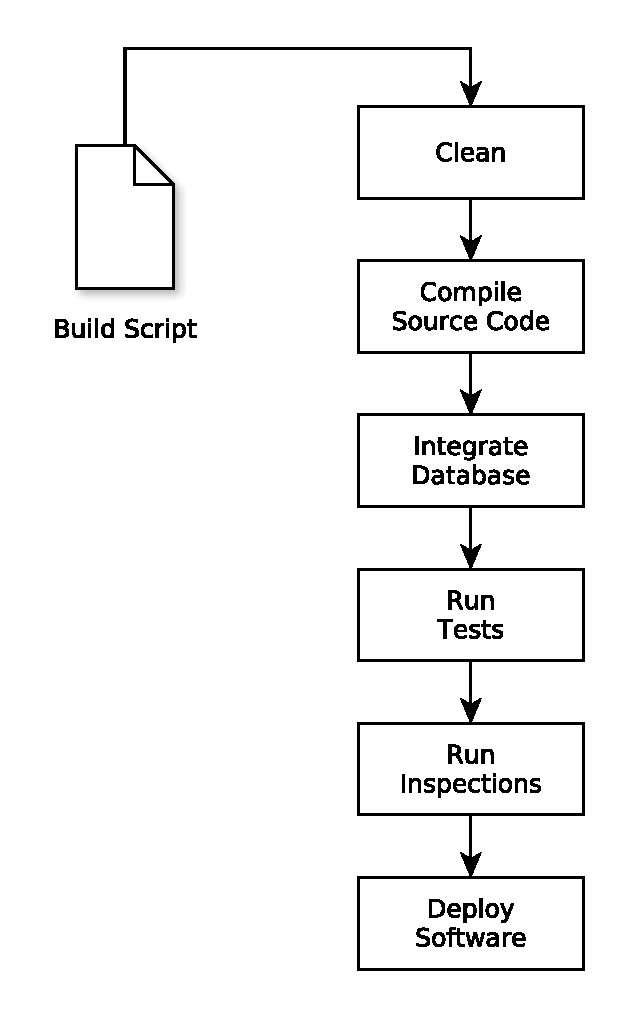
\includegraphics[scale=0.5]{yEd/the_logical_processes_of_a_build_script.eps}
    \caption{The logical processes of a build script \cite{CIbook}.}
    \label{fig:lpobs}
\end{figure}

The whole point of continuous integration is to provide rapid feedback \cite{MartinFowler}. Developers would like to have as fast feedback as possible. To guarantee this quality there are different types of build scripts provided on different roles of requests. Build scripts are divided by the role as lightweight and heavyweight scripts. Lightweight scripts are much more faster than heavyweight scripts. They are used on principle of speed. To ensure this behavior, at first the lightweight scripts are initiated because they can easily catch the basic vulnerabilities and then more advanced tests, inspections, and others are launched by heavyweight scripts which leads to an integration build. Martin Fowler marked the lightweight script which does the first build, as a \uv{commit build} \cite{MartinFowler}. These scripts endeavor for quickness, error detection and software integration, besides that, they also provide a feedback about the results of the whole process to the developer.\\

A script is required due to build automation to provide a \uv{press to build} functionality which is executed many times without any interaction. The script has its logical parts shown on Figure \ref{fig:lpobs}. The transformation process in first part starts with a clean build, what is nothing more than just a clean code compilation. The database integration and the tests execution may be executed differently because of dependence of tests from the database. Not every test depend from the database, due to this, we can divide them and we may run the database independent earlier than the dependent. If there is an error detectable by database independent than it is caught earlier what is more effective according to the time. After this phase, code inspection is launched for further deficiencies. The last stage of the build script is triggered after every previous stages ended successfully. Outcome of this build is an observable result with a log that reflects the build pipeline which forms the basis for the feedback generated for the developers.

%=====================================================================================
\subsection{Research about the Builds of Continuous Integration}
%=====================================================================================

Continuous integration is a practice, not a tool \cite{CollabNet}. Martin Fowler on first of May 2006 stated the basics of CI and the best practices of CI in his article in which he remitted on still popularizing usage of CI. In addition to this article, there was a research provided by a group of scientists about the CI on project provided for the most part from GitHub. Their research is an empirical study about the usage, costs and benefits of CI which are concisely shown in abundant diagrams. The observation of CI and its usage pointed out the significant essential role of CI in open source projects. On the basis of the informations obtained from the researches about the CI, we can make a judgment that this practice will be more and more used in the open source projects. Thanks to automation and standardization, CI helps to effectively prevent errors when deploying applications into operation \cite{CIcure}.\\

Continuous Integration is also referred to as a \uv{cure for human error in deployment} \cite{CIcure} because of error prevention which is rapidly reduced by using this practice. The job of a developer includes a project build repetition which may be also reduced to a few of them for the sense of tasks rate reduction applied on developer. These processes leverage extensive automation and encourage constant code sharing to fix defects early \cite{DigitalOceanCI}. Many of errors, bugs, defects and vulnerabilities are reduced but not every of them is detected by using a CI, but nevertheless the manual software integration is excluded because of CI comprises it as the last step of the software deployment. The impact of the CI usage in software engineering will have extreme demand in the future of IT, more precisely in agile teams using extreme programming technique or any other agile technique. The usage of CI is very adaptive and versatile and it will be more and more used in forthcoming open source projects or any another projects which may not be open source only.\\

In general, if any group of developers would like to use a CI practice, they should fulfill few standards and dwell on these standards. In order for developers to benefit from implementing the practice of CI, they should change their typical day-to-day software development habits \cite{CIQualityFramework}. Usage of CI is beneficial sideline when a developer commits frequently, daily, often, probably few times per day. Farthest, the project should be hosted somewhere on any kid of version control repository which represents a main source for the source code of the product. Besides these two sole development requirements, the expectations are that the developers should not try to commit a broken code. It is avoidable by initiating a private build on their local machine, which decrease the fail chance of the build launched by the CI server.\\

By using CI practice, the risks as software corruption and integration problems are reduced appreciably and any kid of bugs are uncovered quickly. The integration may take unpredictable long time but the use of the CI practice resolve this problem by integrating the software frequently which may result in a few small kind of integration issues. Some other software methodologies integrate their work once after a long time which brings their software to face an incredibly huge integration problem. Martin Fowler pointed this problem in his article: \uv{I was told that this project had been in development for a couple of years and was currently integrating, and had been integrating for several months.} \cite{MartinFowler}. Several articles describe this long time integration as a \textit{Big Bang Integration} \cite{AaltoUniversity}. As we can see on Figure \ref{fig:integration} the risk of the software integration is markedly reduced by using a daily (continuous) integration which is used in a CI practice.

\begin{figure}[H]
    \centering
    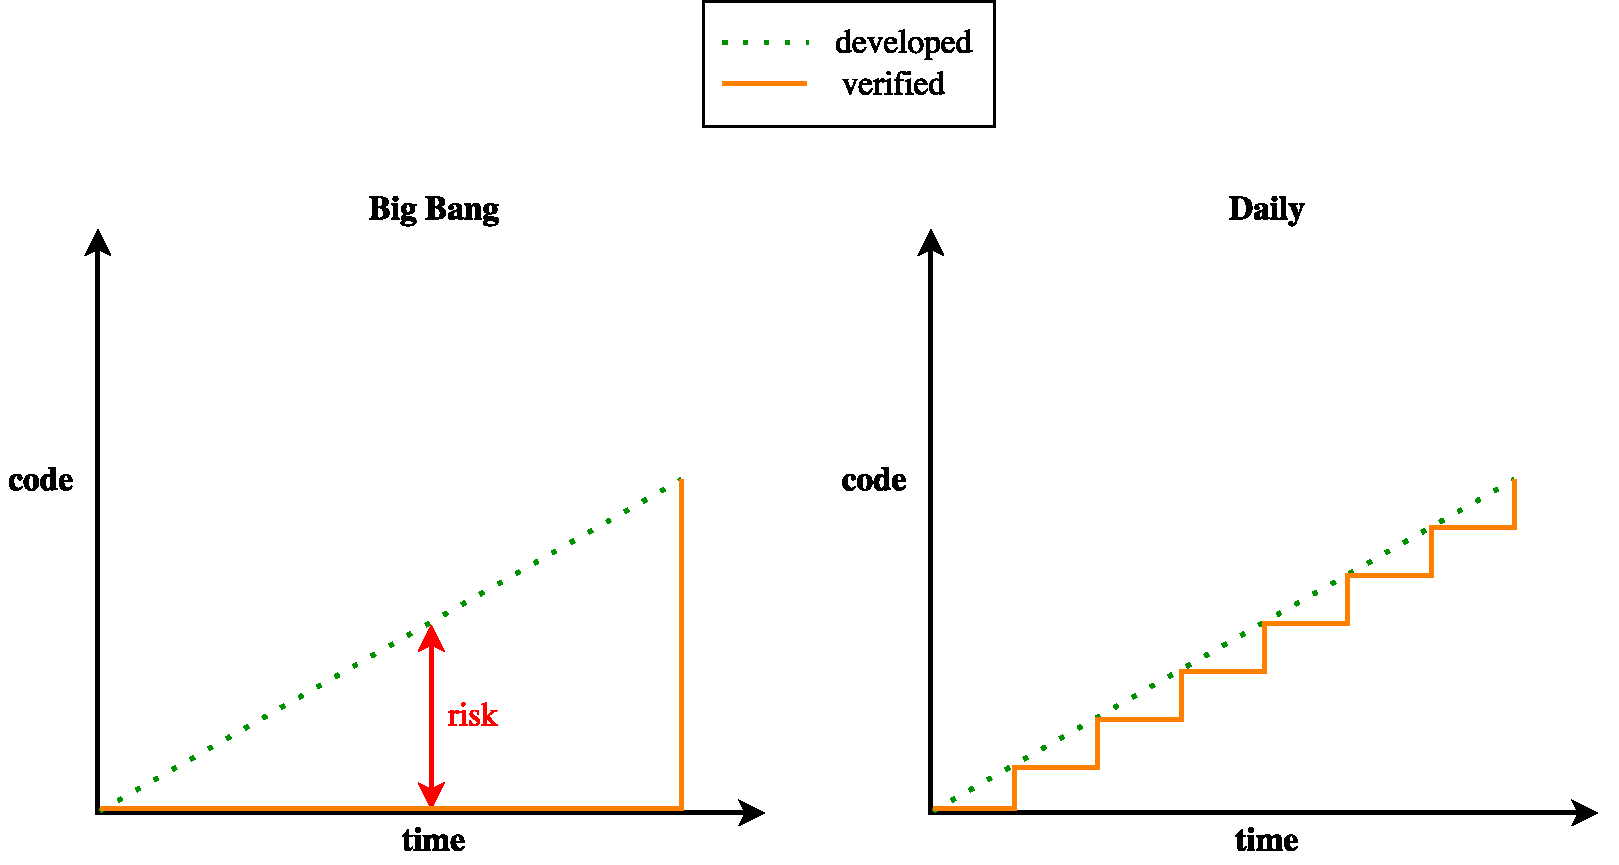
\includegraphics[scale=0.5]{img/big_bang_vs_daily_build.pdf}
    \caption{Comparison of integration builds \cite{AaltoUniversity}.}
    \label{fig:integration}
\end{figure}

%==================================================================================================================
% BEGIN - TODO SECTION

% https://tex.stackexchange.com/questions/53377/inspirational-quote-at-start-of-chapter

{\color{red}TODO: adjust the quote style below, check the citation place}

\textit{\uv{Not integrating continuously is expensive. If you don’t follow a continuous approach, you’ll have longer periods between integrations. This makes it exponentially more difficult to find and fix problems. Such integration problems can easily knock a project off-schedule, or cause it to fail altogether.}}
\hfill ThoughtWorks$^{\tiny{\textregistered}}$ \cite{ThoughtWorks}\\

% END - TODO SECTION
%==================================================================================================================

Prevention against any type of error in a CI is solved via integration build performed on a CI server. Predicting the result of build has drawn the interest of academia and industry \cite{ResultsOfCIbuild}. In term of build result analysis and prediction, most existing studies focused mainly on large software project developed and maintained by big companies \cite{ResultsOfCIbuild}. Travis CI community has created a TravisTorrent\footnote{The name of TravisTorrent was chosen to resemble the close proximity to the GHTorrent project \cite{TravisTorrentWEBPAGE}.} \cite{TravisTorrent} for the purpose of providing a huge amount of information about the builds for full-stack research on continuous integration which is still a developed prototype. Alongside the TravisTorrent, the GitHub company has provided information about the data inside of their version control system in a project called \uv{The GHTorrent project}\footnote{The name signifies a torrent of data coming from GitHub \cite{GHTorrentWEBPAGE}.} \cite{GHTorrent}. Based on these given informations as an open dataset, a few analysis were conducted on them resolving the CI practice in a real life developed projects. The best practices were established on the results of the empirical studies of these obtained data sets provided by many of associations.\\

Studies about the CI were facing against difficult analysis due to inaccessibility of the project's data such as projects of private companies. Due to this, the observations are related to projects mainly hosted on GitHub and predominantly using Travis CI. Informations received from these observations are impressive and they point to the popularizing usage of the CI or promoting CI adoption in projects nowadays. Continuous integration is emerging as one of the biggest success stories in automated software engineering \cite{COPE}.\\

The most interesting question is that how many projects are using the CI at all? In year 2016, an empirical study stated 40\% \cite{COPE} of the projects, observed by them, are using CI practice. Despite of this result, they noted that the number is still in grow and it will be still growing more intensively. While CI is widely used in practice nowadays, we predict that in the future, CI adoption rates will increase even further \cite{COPE}. The results are shown in the Table \ref{table:CI_usage}.

\begin{table}[H]
    \centering
    \caption{Usage of CI in projects \cite{COPE}.}
    \label{table:CI_usage}
    \begin{tabular}{lrr}
        \hline
        Projects Uses CI? & Percentage & Number of Projects \\
        \hline
        Yes               & 40.27\%    & 13,910             \\
        No                & 59.37\%    & 20,634             \\
        \hline
    \end{tabular}
\end{table}

The adoption of the CI to the project may depend in many of factors which includes, for example, familiarity developers with the CI which is the main factor. The median time for CI adoption is one year \cite{COPE}. The basic reason of putting the CI into the development is due to bugs and error reduction, but there is still a possibility to a bug or error incursion into production. As Martin Folwer said \uv{Continuous Integrations doesn't get rid of bugs, but it does make them dramatically easier to find and remove.} \cite{MartinFowler}.

%=====================================================================================
\subsection{Best Practices of Continuous Integration}
%=====================================================================================

The continuous integration practice has become very exploited and its usage has increased considerably the overall agility and efficiency in the development process. It helps stakeholders, testers and product owners to work together seamlessly eliminating bottlenecks and achieve faster time to market \cite{CI-BP1}. This section describes fundamental practices which can lead to dramatical decrease of the costs on the project by using this approach to the CI practices. The costs reduction may be approximately 40\% less as the Ade Miller's study \cite{100DaysOfCI} has shown. The influence may be avowedly known while using these practices. The effort of maintaining the CI system and the usage of the fundamental practices for CI has a magnificent impact on the project. Project investment into a CI can expect to achieve costs reduction, agility growth and error reduction in the development process. Some of the scientific studies report a different count of the CI practices but the general idea of these practices is same in everyone of them. Studies investigate more likely GitHub projects due to the free available informations, from GitHub projects in the GHTorrent and TravisTorrent projects, and on this basis they established these practices.

\subsubsection{Maintain a Central Code Repository}

As a fundamental requirement for the CI is a version control system where is a principal repository held. Software development project involves multiple developers constantly working and pushing code files that need to be orchestrated together to build a product \cite{CI-BP1}. Maintaining a system like this includes a lot of advantages as a source code backup, a reference on the primary mainline of the code with the latest content and a much more other. However, it is mainly used as a source for latest and clean source code of the developed project. This is basic part of the setup for every project developed by a group of people who wish like to share code with the most common way in the development life. Nowadays, it is a often used practice nearly for everybody working on some software product in the development and alongside CI practice it is necessarily used.

\subsubsection{Commit Code Frequently}

The continuous integration is used in agile software development where a huge count of changes are created and quickly integrated into the software product. From this, we can assume, that it points to a frequent code changing. How should we make a recommendation about this to the developers? The essential idea of this practice is to lead the developers to the thought in which they do a little logically compact change which will be committed as fast as they can to the version control repository. A commit should have a characteristic attribute of atomicity which divide the code on two parts as before adjustment and after adjustment. Many of developers do not practice this positive hint of their work. Developers should not wait with the committing of their work after finishing a task given to them. They should commit at least once per day into the baseline and commit a logically comprehensive unit of changes. Version control repositories are based on the source code of the project sharing between developers to accelerate the development process and the developed changes inside of this invokes a CI system which will automatically integrate the change into the software product. A conclusion of this part as a recommendation to the developers may sound like \uv{commit frequently logically comprehensive commits}.

\subsubsection{Do not Commit a Broken Code}

Broken code is a code that contains any type of failure when it is included in a CI build \cite{CIQualityFramework}. A prevention against committing a broken code to the shared code repository there is an opportunity to run a private build on a developer's machine before each one commit. A private build detects the the simplest mistakes such as syntactic error or any other error forgotten in the code which are easy to detect. To reduce the plain error inside of committing code, developer may use a code linter, if a developer is using an IDE\footnote{Integrated Development Environment}, it may has a build in linter. Code linting is a process of running a program which provide a code analysis for potential errors. Some of these basics errors are not detected by linter so this is the reason why a developer should launch a private build before every single change he would like to commit. A private build may include a simple test set to detect these potential error and defects in a created change. To commit a non broken code stands for to run a private build on a developer's local machine before committing his changes. This circumvention may accelerate the change integration.

\subsubsection{Fix Broken Builds Immediately}

An error consequences may beget a broken build as a result of the CI failure. Outcome of this action is an feedback which is sent to the developer as a fix requisition. Developer responsible for this problem should fix it as fast as it is possible irrespective of the build time cost. Fixing a broken build should be the top priority of the project \cite{CIQualityFramework}. As Martin Fowler quoted Kent Beck in his article \uv{nobody has a higher priority task than fixing the build} \cite{MartinFowler}. The meaning of this build fixing is not to stop the actual tasks given to the developers, instead of this, it means to get couple of versed project members to fix the build. CI is effective while the build of the mainline, the principal branch of the project, has a successful termination result. Keeping an operational code in the repository forms the basis of CI which signify a development on a stable based code. Effectiveness of the CI, while the code is stopped at build and not progressing to the integration into the software product, is none. To keep a mainline without broken build is almost always an unfeasible or nearly impossible task due to the human factor. The core idea of this part, how to ensure a mainline without broken builds, is to prioritize the urgent fixes and realize them if needed.\\

Some of the build fix solutions involve dropping the last commit - last change reversion. To avoid broken builds and enhance the solution mentioned before a new practice has been introduced - the pending head. Usage of pending head is a prevention for broken builds of the mainline. A pending head is a way, how to indirectly commit a change into the mainline for the reason of a build make. The result success of the build decides about passing the commit into the mainline.

\subsubsection{Keep the Build Fast}

The stumbling block of the CI practice is the duration time of build. Because the build and test steps must be performed frequently, it is essential that these processes be streamlined to minimize the time spent on these steps \cite{DigitalOceanCI}. Build time may be inappropriately long, what is unacceptable for the developers and can lead to the dysfunction of CI. Every minute you reduce off the build time is a minute saved for each developer every time they commit \cite{MartinFowler}. The most crucial and meaningful solution for reduction of the build duration is inside of the build pipeline. Build is executed by a build script which can be divided into parts which were described in section \ref{build_script}. According to the reduction of the build time, tests took a long enough part of the build time too. A CI practice laboriously rely on the unit test which run approximately equal to core components what makes them very fast. They are the first line of defense in ensuring quality \cite{CI_atlassian}. Vice versa, the API\footnote{Application programming interface} and functional tests are greater time consumers due to their complexity. Graph in Figure \ref{fig:grap_dependence} depicts the dependence of these two factors. A solution of this situation lies in a well chosen pipeline of the deployment, more  precisely, how to run multiple builds in phases properly. When possible, running different sections of the test suite in parallel can help move the build through the pipeline faster \cite{DigitalOceanCI}. A useful consideration of using many of unit tests with high code coverage which have minimal maintenance may also lead the build to time reduction.

\begin{figure}[H]
    \centering
    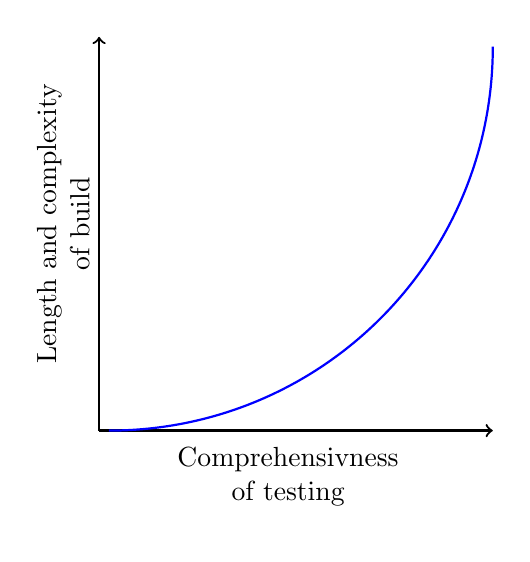
\begin{tikzpicture}[scale=0.5]
        \node[] (i) at (0, 0) {};
        \node[] (l) at (10, 10) {};

        \node[label={[align=center,rotate=90]Length and complexity\\of build}] (left_text) at (0, 5) {};
        \node[label={[align=center]Comprehensivness\\of testing}] (right_text) at (4.8, -2.4) {};

        \draw[draw=black, thick, <-] (10, 0) -- (0, 0);
        \draw[draw=black, thick, ->] (0, 0) -- (0, 10);
        \draw[draw=blue,  thick] (i) to[out=0, in=270] (l);
    \end{tikzpicture}
    \caption{Dependence between length and complexity of the build and comprehensiveness of tests \cite{deployment_automation}.}
    \label{fig:grap_dependence}
\end{figure}

\subsubsection{Everyone can See What is Happening}

Continuous Integration is all about communication \cite{MartinFowler}. Using a CI practice means to share all the gathered informations with the project members. Anybody from the team members should see the informations about the adjustment in the code that somebody had created. But, it is not just about others work, it is about the project state and the changes which have been made inside of it and about the new ones which will be integrated into it.\\

The fundamental part of the CI is the granted feedback about the result of the build realized by the CI server. Feedback is a summary about the log generated 
during build. These informations about the build status should be easy to obtain for anybody ensuring the development speed and quality. Developers must know the status of their adjustment after being handed over to the build. The news in the feedback are very important, especially at some build break. Information obtained from the feedback serve to fine-tune the made adjustment by the creator. Every single build result is assigned to the belonging commit (adjustment) which was made. These informations should be retained for the case if somebody would like to look for a build passing in the past - build passing before the current state. Developers should easily gain these informations and they should be notified if any kind of build broke arose on their work.

\subsubsection{Automate Deployment}

Automating deployment helps to reduce waste \cite{CollabNet}. Automated deployment is nearly adherent to release automation. An essential part of releasing a software product is deploying it, first on development environments, then on QA\footnote{Quality Assurance} and UAT\footnote{User Acceptance Testing} environments, and finally on the real production environment, either on the developing organization's premises, on a customer's premises or on the cloud \cite{deployment_automation}. The usage of the CI required multiple development environments. It comes to this, that you have to move the binaries between multiple environments what follows to create scripts if no manual work is wanted. This allows to deploy application across various heterogeneous environments used in the development process including the final production environment automatedly. In these days there is an interest in virtualization which allow to create the expected environments easy and simple putting together these virtualized environments.\\

If the application meets all standards and criteria it is deployable. Deploying the application into the production signify carefulness you have to pay special attention to. There always was, is and still will be a chance of failure, due to this fact a failure of application deployment requires a rollback. This rollback provide a certain decrease of difficulties about the deployment. Automated deployment, tied into good CI discipline, is essential to making this work \cite{MartinFowler}.

%=====================================================================================
\section{Code Review}
%=====================================================================================

Code review is a substantial part of the development which better the source code quality markedly. The importance of the code review lies in the code enhancement that is significant towards not reviewed code. Code quality is made by imperfection reduction. Analysis of the code by someone else than the author who has different type of view on the code may result in a imperfection detection. The reviewer, who is not the author of the code, can be a person or a software. This reviewer type division involve two types of code reviewing - the automated code review and the non automated review which is done by a developer person. Human person is irreplaceable by a machine but machines do not do mistakes. This is the reason why the development process includes the both type of code review. Automated code review functionality is supported in many of IDEs which inform the developer about the vulnerability in real time. This feature may involve static code analyzing tools which provide extremely fast feedback. Rigby and Bird (2013) find that current software inspection practices tend to converge on Modern Code Review (MCR) \cite{review_participation}. The non automated code review also known as manual code review done by a person via some code review tool. The person is usually a project member who has to known at least the fundamentals about the code what he has to review. Review ends with a code criticism which should be taken by an author positively because of it enhance his code not degrade it. Software code review is a well-established software quality practice \cite{review_participation}. Code review can improve the quality of software products by identifying weaknesses in changes early in the development cycle (Fagan 1999; Shull et al. 2002) \cite{review_participation}.

%=====================================================================================
\subsection{Principle of Code Review}
%=====================================================================================

The resulting work of a person normally involves deficiencies and faults because of the imperfection of people. The amount of imperfections depends from the skills and the experiences of an individual but they are still not removed completely. To catch the rests of non caught vulnerabilities require to examine the work, the source code in case of development, by collaborators or project members. The examination of the work result is called in the development as code review. To understand what is a code review or source code review there are different type of definitions.

\begin{DEF}
Source code review is an act of consciously examining source code intended to find bugs at an early stage of software development \cite{CodeReview_eye_tracking}.
\end{DEF}

\begin{DEF}
Source code review is an offline task aimed at finding the bugs in a code without compiling or executing the code \cite{CodeReview_eye_tracking}.
\end{DEF}

Usage of this practice is reflected on the quality of the source code which is rationally premeditated due to different types of reviewers view. Code review explicitly addresses the quality of contributions before they are integrated into project's code base \cite{CodeReview_quality}. A research article stated that a large portion of faults has been found by only one reviewer \cite{CodeReview_evaluation}. As many of reviewers are participate on a review as many deficiencies of the code are annihilated.

\begin{figure}[H]
    \centering
    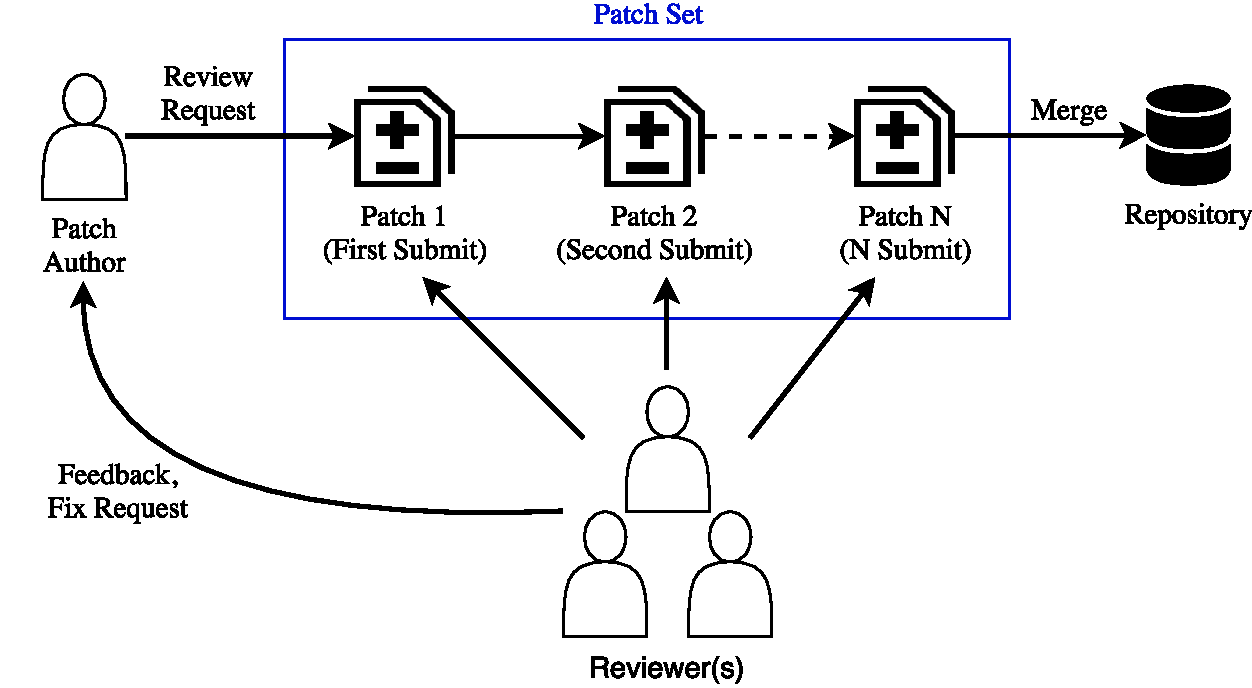
\includegraphics[scale=0.5]{img/process_of_review.pdf}
    \caption{Code review process \cite{CodeReview_IFstatement}.}
    \label{fig:review_process}
\end{figure}

Code review always starts with a request for a review of some patch which is a modification of the actual source code. This patch is reviewed by somebody who has knowledge about this field or it is related to his field in which he is. The reviewer may approve this patch which leads to a merge of patch into the actual source code in the repository - the project code base, or he may request for a fix from the author. This request for a fix does not mean that the patch is impaired, it will enhance the patch instead of patch degradation. After a fix request the process is repeated until an approval. This process in non automated because of it is done by a person or a group of people. In an agile development a thought has arisen which tried to automate this process.

%=====================================================================================
\subsection{Types of Code Review}
%=====================================================================================

There are many of code review types depending from the aspect, view and the review provider. Code review types can be also {\color{red}xxx} or automated. The {\color{red}xxx} is {\color{red}yyy}. The automated code review is based on a predefined set of rules which are checked by a software whether the conditions are met or not.\\

{\color{red}TODO: phrase for <non automated code review>}

%=====================================================================================
\subsection{Automated Code Review}
%=====================================================================================

Abcd.

%=====================================================================================
\chapter{Continuous Integration in Open Source Projects}
%=====================================================================================

Abcd.

%=====================================================================================
\section{Open Source}
%=====================================================================================

Abcd.

%=====================================================================================
\section{Github}
%=====================================================================================

Abcd.

%=====================================================================================
\section{TravisCI}
%=====================================================================================

Abcd.

%=====================================================================================
\section{ManageIQ}
%=====================================================================================

Abcd. \url{https://lwn.net/Articles/680060/}

%=====================================================================================
\chapter{Implementation}
%=====================================================================================

Abcd.

%=====================================================================================
\section{ManageIQ Bot}
%=====================================================================================

Abcd.

%=====================================================================================
\section{Pronto}
%=====================================================================================

Abcd.

%=====================================================================================
\section{Request for a Pull Request Review}
%=====================================================================================

Abcd.

%=====================================================================================
\chapter{Conclusion}
%=====================================================================================

Asdf.
